\section{PTC thermistors}
As aforementioned, a positive temperature coefficient thermistor is a thermally sensitive resistor that varies its resistivity as the temperature of the environment changes. Particularly because it is a positive coefficient, as the temperature increases, the resistivity of the semiconductor device increases as well.

\subsection{Charateristics}
One of the most important properties of the PTC thermistor is the characteristic curve between the \textbf{resistance} $R$ and the \textbf{temperature} $T$, which has to be converted from Celsius (or Fahrenheit) to Kelvin. Its curve is a positive exponential graph that respects the following equation \cite{Saburi196353}:

\begin{equation*}
    R = R_0\,e^{\beta\,(\frac{1}{T} - \frac{1}{T_0})}
\end{equation*}

\noindent Where $R$ is the calculated resistance at the temperature $T$ and $R_0$ is the resistance measured at temperature $T_0$. The coefficient $\beta$ is the thermistor constant and it depends on the materials used to build it and on the thermistor dimensions. It is possible to obtain this value by measuring its resistance value at two different temperatures and computing the following equation \cite{Saburi196353}.

\begin{equation*}
    \beta = \frac{\ln{\frac{R_2}{R_1}}}{\frac{1}{T_2} - \frac{1}{T_1}}
\end{equation*}

\noindent Using the previous equations, the curve can be plotted by writing down the equations using MATLAB, or other programming languages. Figure \ref{fig:PTC_logarithmic} shows how much the resistance increases as the temperature increases. In this case, the coefficient $\beta$ has been calculated by assuming that when $T_1 = 273.15 K$, $R_1 = 1k\Omega$ and when $T_2 = 373.15 K$, $R_2 = 100M\Omega$.\footnote{Please be aware that the selected values are purely for illustrative purposes; no devices with these characteristics exist in reality}

\begin{figure}[h]
    \centering
    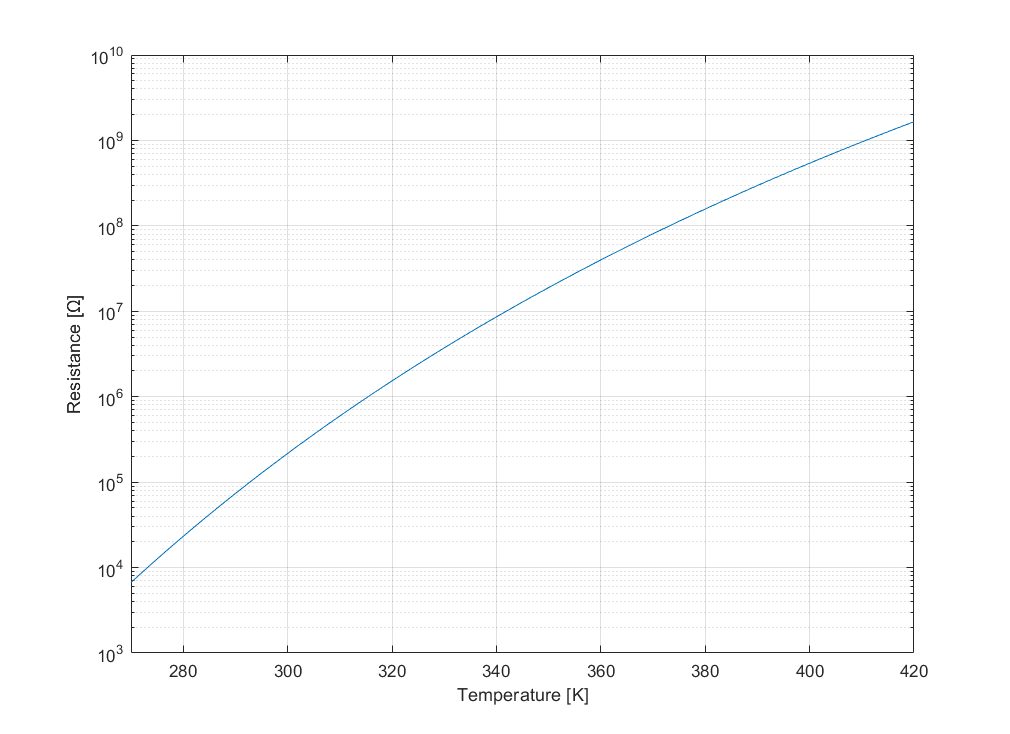
\includegraphics[width = .7\textwidth]{../res/plots/PTC_logarithmic.png}
    \label{fig:PTC_logarithmic}
    \caption{PTC resistance-temperature logarithmic curve.}
\end{figure}

\FloatBarrier\noindent Secondly it might be interesting to plot the change ratio between the resistance $R$ and the value of the resistance at some fixed temperature. In the figure \ref{fig:PTC_ratio}, the fixed temperature value $T_0$ was 25° celsius (or 298.15 Kelvin) which implies that $R_0 = 16.7 k\Omega$.

\begin{figure}[h]
    \centering
    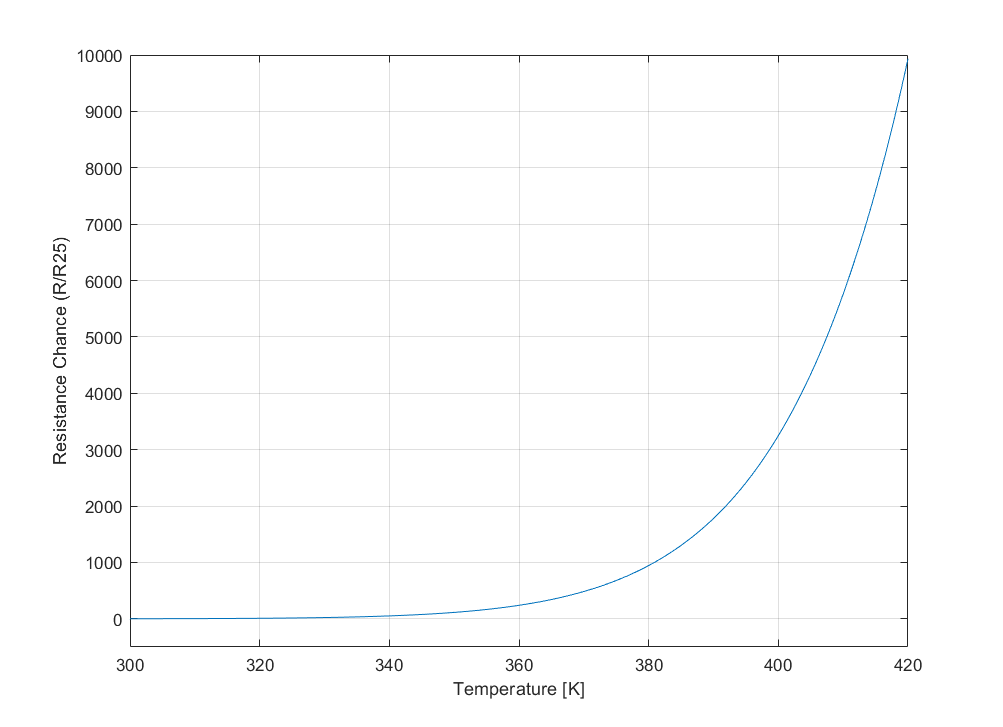
\includegraphics[width = .7\textwidth]{../res/plots/PTC_ratio.png}
    \label{fig:PTC_ratio}
    \caption{PTC change ratio between $R$ and $R_0$}
\end{figure}

\FloatBarrier\noindent In both of the plots the resistance value or the change ratio drastically increases as the environment gets hotter. In the next paragraph, we will see how important this characteristic is for building current-regulating circuits and protecting delicate components.

\todo{V - I characteristic curve}

\todo{other aspects like the dissipation constans, noise, long term stability}


\subsection{Applications}





